
%
% latex-sample.tex
%
% This LaTeX source file provides a template for a typical research paper.
%
%
% Use the standard article template.
%
\documentclass{article}
\usepackage{textcomp}
\usepackage{float}

% The geometry package allows for easy page formatting.
\usepackage{geometry}
\geometry{letterpaper}

% Load up special logo commands.
\usepackage{doc}

% make a reference to Hypertext 
\usepackage{hyperref}

% Package for formatting URLs.
\usepackage{url}

\usepackage{listings}

% Packages and definitions for graphics files.
\usepackage{graphicx}
\usepackage{epstopdf}
\DeclareGraphicsRule{.tif}{png}{.png}{`convert #1 'dirname #1'/'basename #1 .tif'.png}

%
% Set the title, author, and date.
%
\title{Group 1  \\ \small{DNSC 6211: Programming for Analytics}}
\author{
	Suffyan Asad \\
	Yiran Ding \\
	Paola Quijano\\
}
\date{December 9 of 2015}

%
% The document proper.
%
\begin{document}

% Add the title section.
\maketitle

% Add an abstract.
\abstract{
Describe your project within 200 words.  One way is answer the following questions regarding your project: (a) what did you do? (b) why did you choose do that? (c) how did you go about doing your project (d) what did you find out?, and finally (e) What did you find out? The content of your abstract and the outline and contents of your report may vary according to the needs of your specific research topic.
}

% Add various lists on new pages.
\pagebreak
\tableofcontents


% Start the paper on a new page.
\pagebreak

%
% Body text.
%
\section{Introduction}
\label{introduction}

Billboard is a music magazine, which provides rankings of trending and popular songs based on weekly sales, radio play and online streaming.  Based on this information, our group was interested in analyzing how people think about popular songs once they have been on Billboard\textasciiacute s Top 100 hits list. Will people still be positive about an old popular song? Will they still be talking about it? In other words, is the ranking still making sense after a few years? 

By means of answering these questions, we decided to run a sentiment analysis, with the help of Twitter, which required the use of natural language processing and text analysis, in order to give a positive/negative score to the data collected from the social media. With the analysis, we were able to see the correlation between high ranked song and their positive or negative effect throughout social media. 

\section{Background \& Method}

The Billboard Hot 100 is the music industry standard record chart in the United States for singles, published weekly by Billboard magazine. As mentioned before Billboard generates the top 100 song based on a ratio of (35-45 \%) targets sales (physical and digital), airplay (30-40\%) and streaming (20-30\%)\cite{billboard}. In order to run our project we started by looking for a public and free ranking dataset, from Billboard website, to use as reference.  We ended up obtaining a total of 180 songs from the list of the top 20 songs for each year from 2006 until 2014.

Likewise, in order to be able to ran the sentiment analysis, we had to search for a dataset which contained comments about our songs list. We mainly wanted a popular dataset with a convenient API, in order for us to get the data easy for analysis. The first option was Facebook, however Facebook stopped providing the Hashtag API free for private users, so we ended up with the Twitter dataset and its Python interface. With Twitter we took 40 tweets from each song, so that we could look for positive and negative tweets, as our main question was understanding if there was a correlation between the age of the song and the number of tweets(we mean by  age, the amount of years since the song was part of the list).  Then with the help of SQL, we were able to run queries on our dataset and find the different relations between the age of the song and the amount of positive tweets, negative tweets and retweets. Finally R gave us the tools to run linear regressions in the different models and enabled us to create graphs in order to visualize the results


\section{Organization}

The whole group contributed by deciding the main topic and the use of each tool.  Yiran did the web scraping of billboard list into python and contributed to the write up, Suffyan did the sentiment analysis, run the queries in mySQL and rshiny, Paola did the conclusions and analysis of the results, contributed with the write up and created the Latex draft

\subsection{Workflow}
\begin{enumerate}
\item We began Web-Scraping the data from Billboard into Python, and created a list of songs. We scraped top 20 songs from the top 100 of year 2006, 2007, 2008, 2009, 2010, 2011, 2012, 2013 and 2014.
\item For each song saved in the Python Billboard ranking list, we retrieved relative data from Twitter using API. 
\item We first saved the users profile information in order to have the country of origin, which was used to create the heat map
\item We created two lists for text analysis and run the sentiment analysis, saved the positive and negative score for the data and created a database with the use of MySql. 
\item With MySql we ran queries in order to retrieve significant data that enabled us to analyzes the data and create plots for analysis
\item With the help of packages as rworldmap and ggplot2, R enabled us to create plots of the analysis and plot the map for geographic analysis. 
\item Finally, we designed a shiny app which allows to choose any year between 2006 and 2014  and see the analysis by song and year. 
\end{enumerate}
 \begin{figure}[H]
  \centering
  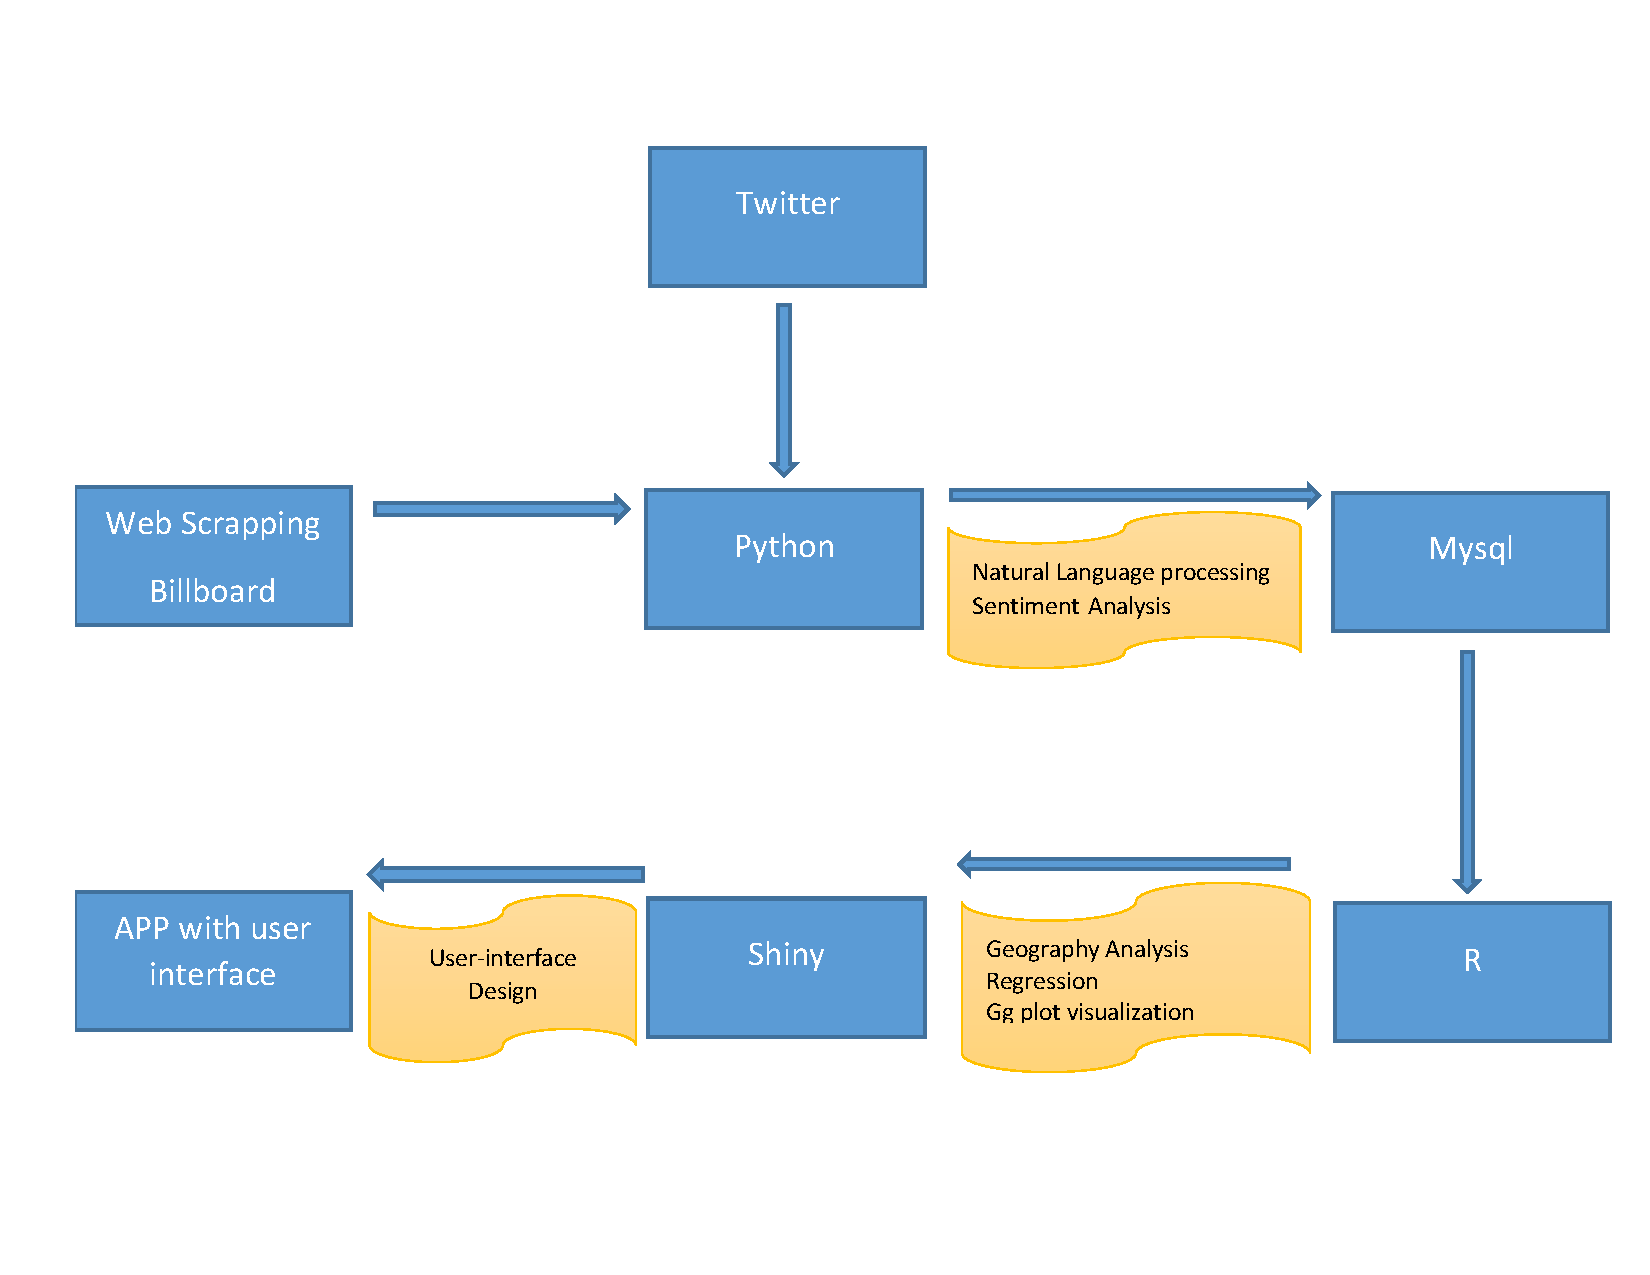
\includegraphics[scale=0.6]{WorkFlowGraph.pdf}
  \caption{The project workflow}
\end{figure}

The whole process is reproducible by our code, however it will take a few hours to retrieve data from Twitter.  We attached the database in MySql if you are interested in reproducing our analysis without going through difficulties of limitations that may be driven by Twitter API. Pleas make sure to install "rworldmap" package to use it.

\begin{lstlisting}[frame=single]
install.packages("rworldmap")
\end{lstlisting}

\subsection{Project structure}
We took the top 20 songs for each year since 2006 until 2014 from Billboard website. These songs have been a success in the music industry, so we wanted to know if people are still commenting about this songs even if they had been a success years before.  We mainly looked for a correlation between the age and the ranking of the song. To analyze this situation, we took the songs and saved the main information as name and artist into a database.  We then took 40 tweets from each song with the help of Python Twitter API, which allowed us to search for specific tags from recent Tweets, to exactly match the list of songs we retrieved from  Billboard. We were able to create a ranking list from the positive score estimated by the tweets and compare it with original ranking of each 20 songs. And finally we were able to retain the original location of the twitter user in order to make a geographic analysis using R.

\subsection{Files and Steps}
Following are the steps that can be used to recreate the results:

\subsubsection{Listing and Purpose of script files}
\begin{enumerate}
\item \textbf{"BillboardScraper.py": } This file scrapes the top 20 songs along with their artist and ranking from billboard for the given years and creates a table in the database containing them.
\item \textbf{"TwitterSentimentAnalyzer.py": } This file takes the songs stored in the database by the previous script, and gets the tweets on them, and performs the sentiment analysis to score the tweets, and get the number of rwtweets. Additionally, for each tweet, his location is taken from the user information sent with each tweet by Twitter, and from that, using the GeoNames API, the country is retrieved.
\item \textbf{"positive-words.txt"} and \textbf{"negative-words.txt": } These are the list of positive and negative words given professor in the Programming for Analytics class. They contain a list of positive and negative words used to judge the sentiment of the tweets.
\item \textbf{"ProjectApp" (Folder): } This folder contains the ui.R and server.R of the R Shiny Application used to explore the results year by year and to display the charts in detail.
\item \textbf{"dbScript.sql" :} This is the SQL script file used to re-create the database as generated by running \textbf{BillboardScraper.py} and \textbf{TwitterSentimentAnalyzer.py} quickly, since running the two files instead of the script file can take upto an hour or more.
\end{enumerate}

\subsubsection{Original Workflow}
Following is the workflow we followed in our working. It is time consuming and can take over an hour.

\begin{enumerate}
\item create database called SongsDb in MySQL.
\item created a profile on GeoNames API (the profile username is in the code, and but it has a limit of 15,000 reverse GeoMapping calls per day, and this analysis uses 7200 of the allowed calls in each run). \href{http://www.geonames.org/login}{GeoNames Login/Register page}
\item run BillboardScraper.py
\item run TwitterSentimentAnalyzer.py
\item run the R Shiny Application
\end{enumerate}

\subsubsection{Alternate workflow, (Quicker, recommended for evaluation}
\begin{enumerate}
\item run dbScript.sql file
\item run the R Shiny Application
\end{enumerate}


\subsection{Figures and Tables}

On Figure 2 we can see the linear regression of the  Positive score and the age of the song. From the figure we can see that when the age increases, there is a slightly decrease in the positive score of the song. Generally, people still express a positively feeling about the song after a few years. However there is a trend that the positive score goes down a little bit as time goes by.

\begin{figure}[H]
  \centering
  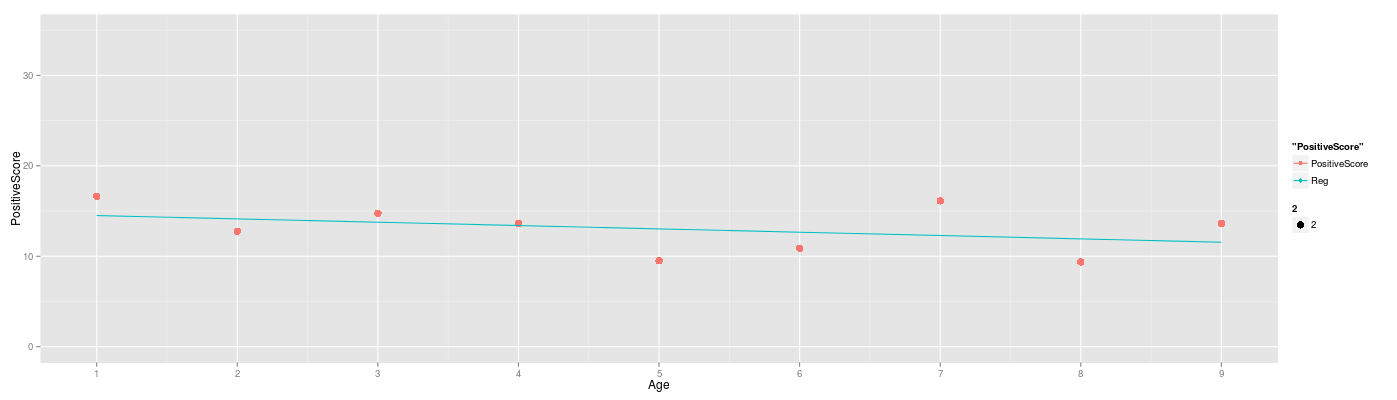
\includegraphics[scale=0.3]{reg_Age_PostitveTweets.png}
  \caption{Linear Regression Age vs Possitive Tweets}
\end{figure}


On Figure 3 we can see the linear regression of the number of retweets in the relation of age. When the age of the song increase, the number of retweets goes up. People are more likely to retweet about an old song when it recalls the good memory of it.

\begin{figure}[H]
  \centering
  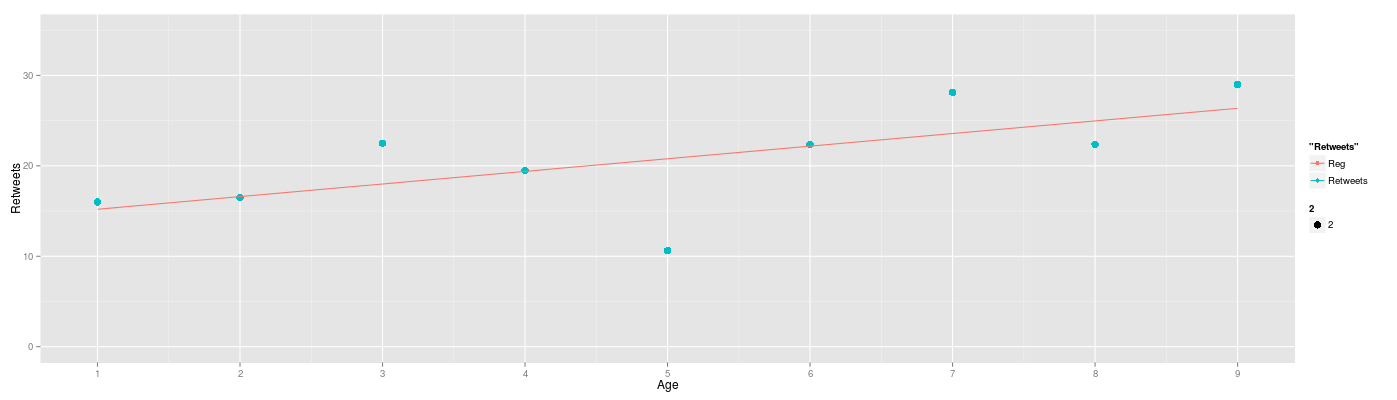
\includegraphics[scale=0.3]{reg_Age_Retweets.png}
  \caption{Linear Regression Age vs Retweets}
\end{figure}




\begin{figure}[H]
  \centering
  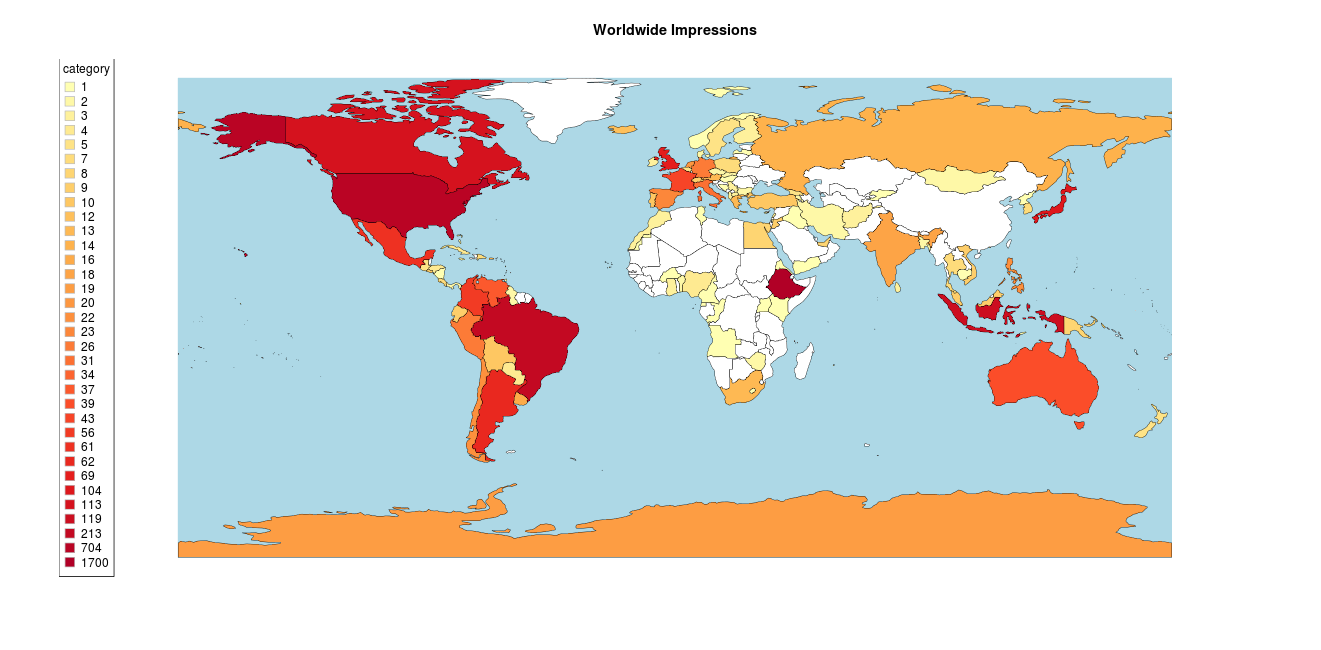
\includegraphics[scale=0.3]{worldwide_impressions.png}
  \caption{Worldwide Impressions}
\end{figure}

We did find some interesting result from figure 4, which is the world map with its impression about the song. The darker red indicates the number of impressions done by a user from certain country. United States and UK is as expected on the Top 10 in this index, since twitter and Billboard are very popular in these regions. However, UK is only the 7th in the index, and we were surprised that Ethiopia has a very high positive score in the index.  We will have more discussion and conjecture for this interesting phenomenon.
\begin{figure}[H]
  \centering
  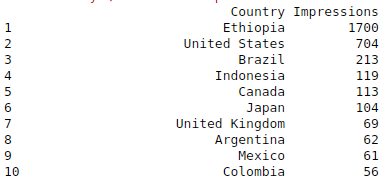
\includegraphics[scale=0.3]{top_10_countries.png}
  \caption{Top 10 Countries}
\end{figure}
Figure 6 shows the table with the correlation of the variables age, positive tweets, negative tweets, positive score, negative score and retweets.  We can see from it that there is a strong positive correlation between the age of the song and the retweets.
\begin{figure}[H]
  \centering
  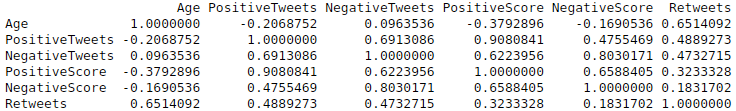
\includegraphics[scale=0.3]{Correlation.png}
  \caption{Top 10 Countries}
\end{figure}

\section{Discussion}
\subsection{Learnings \& Challenges}


The project was made more challenging as we found some limitations in various aspects:
\begin{itemize}
\item One of the steps of the project was to realize a reverse Geocoding, in order to find the user's location, specifically the country.  In this case one of the biggest limitations was that Google API only allowed 2500 searches per day and in its Terms and Conditions it was required to display data using Google Maps, that is why we took the decision to work on GeoNames, as it is a very powerful database that contains data from each country and it has a limit of 15000 searches per day, 7 times more than Google.

\item In some cases we were not able to reverse some locations in order to find the country of origin, as users sometimes do not write accurate information in their Twitter account, this could have happened maybe by mistake or just because of fun by the user.

\item Some of the songs titles had words that denoted positive or negative words so when doing the sentiment analysis we were not able to identify if it was a positive or negative tweet, given the title, so we decided to remove those songs from the list.

\item We also wanted to use the Facebook API as another source, but unfortunately it is no longer available to do searches, so we had to limit the search to Twitter.

\item One of the challenging parts of the project was based on deciding the amount of tweets to search, as GeoNames allowed to search on 15000 per day, we decided to do sentiment analysis to at most 40 tweets per song.

\item As Shiny was a new application for us we found it very challenging to work on.

\item The data obtained from Twitter was very recent as they only allow to obtain data from at most 7 days.

Finally, one the most interesting things we found on the project was that when we plotted the world heat map, we saw that Ethiopia had been very active since 2006. We were not able to explain the reason why this happened, but would have liked to explore a little bit more the reason of the high rate of tweets.  Our hypothesis were:
\begin{itemize} 
\item Ethiopia may have a city that matches a US city.
\item Users may think adding Ethiopia can be fun as an original location.
\item Basically this are genuine tweets.  
\end{itemize}
\end{itemize}
\pagebreak


\section{Conclusion}

To focus the conclusion of our analysis, let's take a look at Figure 2, Age vs positive tweets, in this case we can see a small negative slope, which means a negative relationship between the positive tweets and the age of the song.  As expected people keep talking about old hit songs but in a less rate compared to the newer songs, people will remember and talk about a newer song more easily compared to an older songs.  We can even see the result on Figure 6, which shows the table with the respective correlations.

On the contrary, on Figure 3 we can see the amount of retweets is higher for older songs, the graph shows a positive relationship between the age of the song and the amount of retweets. People will have a positive thought, as it may bring a good memory, about an old song when it is recalled by someone else. And will be more attracted to share their positive thought by retweeting the post to friends and followers.

Figure 7 below shows the relation between the age of the song and the sentiment analysis done. We can confirm by these graph as well, that as the songs are older it is more likely for people to retweet about it.
\begin{figure}[H]
  \centering
  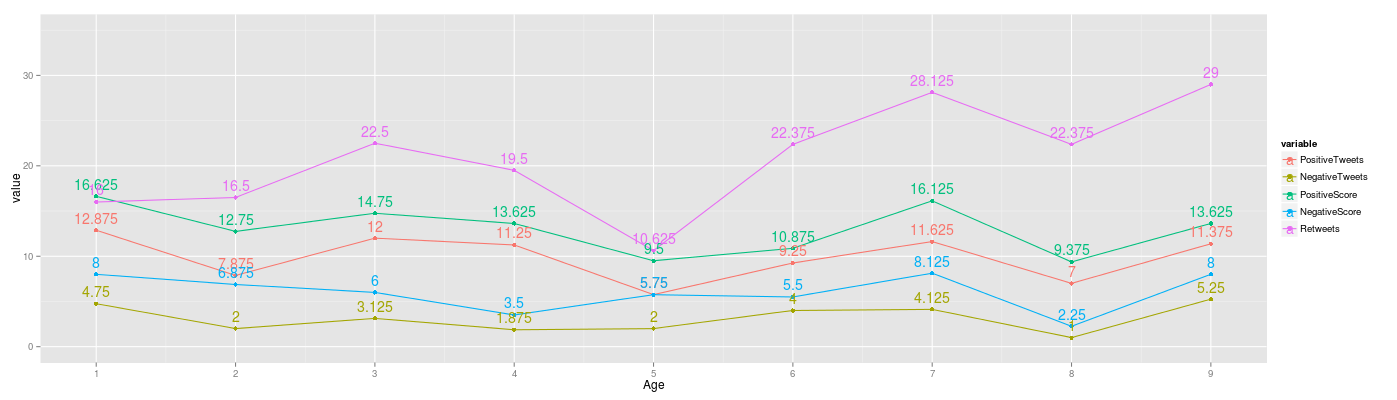
\includegraphics[scale=0.3]{Stats_by_Age.png}
  \caption{Stats by Age}
\end{figure}


\begin{thebibliography}{9}

\bibitem{rproject} 
The R Journal
\\\texttt{https://journal.r-project.org/archive/2011-1/RJournal\_2011-1\_South.pdf}

\bibitem{stackoverflow} 
Stackoverflow rworldmap example
\\\texttt{stackoverflow.com/questions/11225343/how-to-create-a-world-map-in-r-with-specific-countries-filled-in}

\bibitem{billboard} 
Billboard Hot 100
\\\texttt{https://en.wikipedia.org/wiki/Billboard\_Hot\_100}

\bibitem{TwitterAPIRef}
Twitter API Reference
\\\texttt{https://dev.twitter.com/rest/reference/get/search/tweets}

\bibitem{GeoNames}
Geo Names API Reverse Geocoding Reference
\\\texttt{http://www.geonames.org/export/web-services.html\#countrycode}

\end{thebibliography}

\end{document}


